\chapter{Related Work} 
\label{ch:relatedwork}

% This chapter should include a broad and detailed review of relevant existing
% work. The literature review
% should provide background and context for the thesis work. The subsections may be organized in whatever
% manner seems best suited to the material---chronological, or by topic, or
% according to some other criteria (e.g., primary versus secondary resources).

Automated fault localization in general and more specifically spectrum based
fault localization have extensive literature exploring the different approaches
to facilitate debugging and increase developer efficiency. Considering that
AFLuent relies on many concepts developed by this literature, this section will
explore and discuss how past work shapes AFLuent. Several sections are created
to for specific area of literature.

\section{Automated Fault Localization}
\label{sec:AFLlit}

Survey papers are one of the many ways that assist in better
understanding and having a wide collection of the existing
literature surrounding automated fault localization (AFL).
Wong et al. \cite{wong2016survey} explores the variety of AFL approaches and
surveys research completed in that area between 1977 and 2014. The survey paper finds and
discusses more than 334 different papers in many approaches in AFL.
\begin{figure}[!htb]
	\begin{center}
		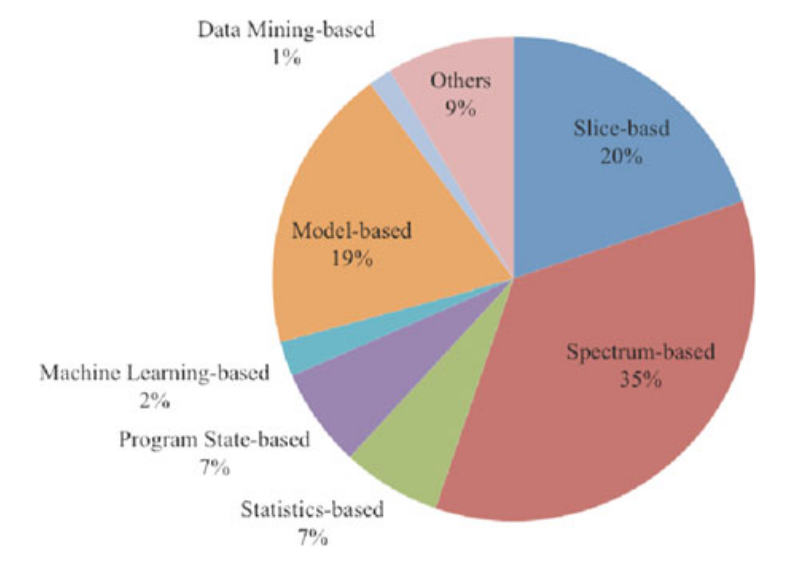
\includegraphics[width=10cm]{wong_pie_chart.png}
		\caption{\label{fig:wong_breakdown} AFL papers found by Wong et al. \cite{wong2016survey}}
	\end{center}
\end{figure}

A breakdown of the found research is shown in Fig. \ref{fig:wong_breakdown}, where the
majority of found papers are focused on Spectrum-Based Fault Localization (SBFL).
Overall this research provides a great
starting point to find and compare the different types and approaches of AFL.
Another benefit of this resources is that
Wong et al. \cite{wong2016survey} expands on the types of SBFL
and reviews key literature that contributes show the benefits and drawbacks of
each approach.

\subsection{SBFL Approaches}
\label{subsec:sbfl}

\subsubsection{Similarity Coefficient Based Technique}
\label{subsubsec:coefficient_based}

One of the most relevant SBFL techniques described by Wong et al.
\cite{wong2016survey} is similarity coefficient based ones. Generally, these approaches
seek to quantify how close ``the execution pattern of a statement is to the
failure pattern of all test cases'', where the the closer they are the more
likely that this statement to contain the error. In order to create a
measurement of closeness, several equations have been developed and evaluated by
past literature. Fig. \ref{fig:sbfl_eq} shows some of the equations reviewed by
Wong et al in, however, more popular formulas have been developed that
required the developer to analyze less code before finding the fault. Despite
the existence of many Similarity Coefficient formulas, Yoo et al.
\cite{yoo2014no} concludes in an extensive evaluation study that there is no
formula that outperforms all others in all circumstances. With that in mind,
AFLuent gives the user the option to choose which approach to use and includes
a performance evaluation of each.

\begin{figure}[!htb]
	\begin{center}
		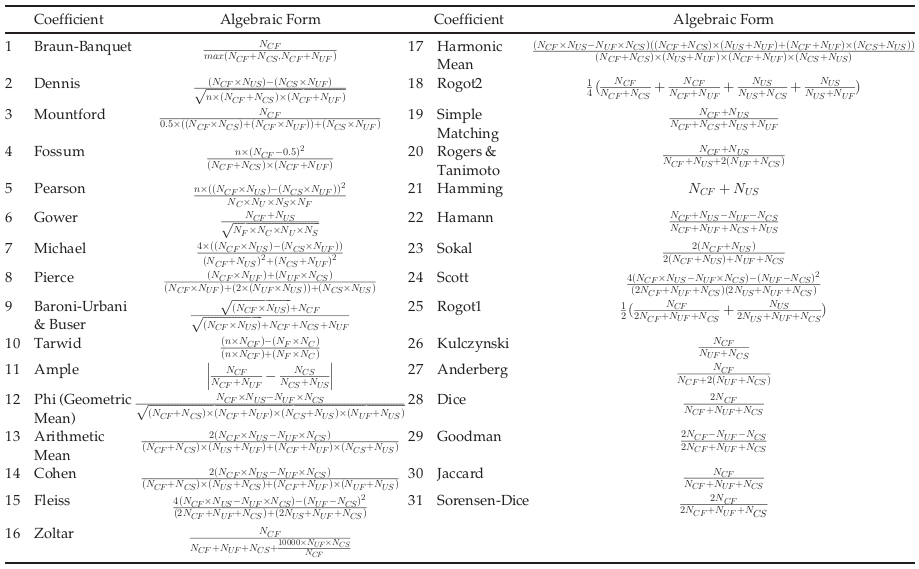
\includegraphics[width=\textwidth]{sfl_table.png}
		\caption{\label{fig:sbfl_eq} Coefficient Based Formulas \cite{wong2016survey}}
	\end{center}
\end{figure}

\subsubsection{Tarantula}
\label{subsubsec:tarantula_lit}

Starting off with the Tarantula formula (fig. \ref{fig:tarantulaEquation}), it's
one of the foundational equations that was introduced to attempt to visualize
suspicious statements using color ranges \cite{jones2002viz,
Jones2005TarantulaEval}. A tool using this equation was also implemented in Java
in order to scan code and assign colors to statements based on their
suspiciousness. The equation for Tarantula is made of two main ratios, the first
one being the number of failed tests that cover the element divided by the total
number of failed tests (\(\frac{\textbf{N$_{CF}$}}{\textbf{N$_{CF}$ +
\textbf{N$_{UF}$}}}\)). The other ratio used is number of passing tests that
cover the element divided by total number of passing tests
(\(\frac{\textbf{N$_{CS}$}}{\textbf{N$_{CS}$}+\textbf{N$_{US}$}}\)).
The equation is then assembled as seen in fig. \ref{fig:tarantulaEquation}.
To better understand how the equation works, we can look at the important terms
that have the largest influence in changing the output.The number of failed
tests that cover the element is clearly the main influencer here because it's
what causes the numerator to grow larger. This means that an increase in failed
tests that cover the element cause an increase in suspiciousness. Additionally,
a decrease in the number of failing tests that do not cover the element also
increase suspiciousness. Considering these two points, Tarantula gives a better
indicator of suspiciousness when there are fewer failures in tests covering
elements not under inspection. In addition to the logical analysis of the
equation previous works provide an empirical evaluation of Tarantula in
comparison to other formulas. Jones et al. \cite{Jones2005TarantulaEval}
compares the effectiveness and efficiency of Tarantula to techniques such as Set Union, Set
Intersection, and Nearest Neighbor. The results demonstrate that Tarantula
outperform the other Techniques where it provided a better guidance to the
developer. Using Tarantula a developer would need to manually
inspect fewer elements of the program compared to when using other approaches.

Another variation of Tarantula is also introduced in \cite{debroy2010grouping},
where grouping of suspicious elements is used to provide a better guide for
developers. In this modification, ``statements that are executed by the same
number of failed test cases are grouped together'', then suspiciousness scores
are used to sort elements within each group. By doing so, two layers of sorting
exist, the first one based on the number of failed tests covering the element,
and then the suspiciousness scores. The empirical results in Debroy et al.
\cite{debroy2010grouping} show a statistically significant improvement provided
by this grouping technique where the developer need to review less elements and
more faults are accurately detected. While Debroy et al. only applied the
grouping technique to Tarantula and a neural network-based approach, it could be
extended to include other similarity coefficient based techniques.

Overall, while other formulas outperform Tarantula as will be discussed,
incorporating this equation in AFLuent offers a starting point and a point of
comparison to other equations. One of the goals of AFLuent is to give the user
the ability to choose their most fitting approach to localize faults, and it's
useful to include Tarantula as one of the available options.

\subsubsection{Ochiai}
\label{subsubsec:ochiai_lit}

\subsubsection{DStar}
\label{subsubsec:dstar_lit}

\subsubsection{O and \textbf{$O^p$}}
\label{subsubsec:o_lit}

\subsection{Combining Approaches}
\label{subsec:combining_approaches}

While AFLuent does not rely on non-SBFL approaches in its implementations, it's
useful to explore other methodologies that could assist in the debugging
process. This creates a guide for potential extendibility of AFLuent and
provides a way to fill in the shortcomings of AFLuent.
% TODO: develop more using "Search-based fault localization" and "Learning to Combine Multiple Ranking Metrics
% for Fault Localization"

\section{Existing Tools}
\label{sec:existing_tools}

\section{Usability and Accessibility}
\label{sec:usability_accessibility}

